% Options for packages loaded elsewhere
\PassOptionsToPackage{unicode}{hyperref}
\PassOptionsToPackage{hyphens}{url}
%
\documentclass[
  8pt,
  ignorenonframetext,
]{beamer}
\usepackage{pgfpages}
\setbeamertemplate{caption}[numbered]
\setbeamertemplate{caption label separator}{: }
\setbeamercolor{caption name}{fg=normal text.fg}
\beamertemplatenavigationsymbolsempty
% Prevent slide breaks in the middle of a paragraph
\widowpenalties 1 10000
\raggedbottom
\setbeamertemplate{part page}{
  \centering
  \begin{beamercolorbox}[sep=16pt,center]{part title}
    \usebeamerfont{part title}\insertpart\par
  \end{beamercolorbox}
}
\setbeamertemplate{section page}{
  \centering
  \begin{beamercolorbox}[sep=12pt,center]{part title}
    \usebeamerfont{section title}\insertsection\par
  \end{beamercolorbox}
}
\setbeamertemplate{subsection page}{
  \centering
  \begin{beamercolorbox}[sep=8pt,center]{part title}
    \usebeamerfont{subsection title}\insertsubsection\par
  \end{beamercolorbox}
}
\AtBeginPart{
  \frame{\partpage}
}
\AtBeginSection{
  \ifbibliography
  \else
    \frame{\sectionpage}
  \fi
}
\AtBeginSubsection{
  \frame{\subsectionpage}
}
\usepackage{amsmath,amssymb}
\usepackage{lmodern}
\usepackage{iftex}
\ifPDFTeX
  \usepackage[T1]{fontenc}
  \usepackage[utf8]{inputenc}
  \usepackage{textcomp} % provide euro and other symbols
\else % if luatex or xetex
  \usepackage{unicode-math}
  \defaultfontfeatures{Scale=MatchLowercase}
  \defaultfontfeatures[\rmfamily]{Ligatures=TeX,Scale=1}
\fi
% Use upquote if available, for straight quotes in verbatim environments
\IfFileExists{upquote.sty}{\usepackage{upquote}}{}
\IfFileExists{microtype.sty}{% use microtype if available
  \usepackage[]{microtype}
  \UseMicrotypeSet[protrusion]{basicmath} % disable protrusion for tt fonts
}{}
\makeatletter
\@ifundefined{KOMAClassName}{% if non-KOMA class
  \IfFileExists{parskip.sty}{%
    \usepackage{parskip}
  }{% else
    \setlength{\parindent}{0pt}
    \setlength{\parskip}{6pt plus 2pt minus 1pt}}
}{% if KOMA class
  \KOMAoptions{parskip=half}}
\makeatother
\usepackage{xcolor}
\newif\ifbibliography
\setlength{\emergencystretch}{3em} % prevent overfull lines
\providecommand{\tightlist}{%
  \setlength{\itemsep}{0pt}\setlength{\parskip}{0pt}}
\setcounter{secnumdepth}{-\maxdimen} % remove section numbering
\newlength{\cslhangindent}
\setlength{\cslhangindent}{1.5em}
\newlength{\csllabelwidth}
\setlength{\csllabelwidth}{3em}
\newlength{\cslentryspacingunit} % times entry-spacing
\setlength{\cslentryspacingunit}{\parskip}
\newenvironment{CSLReferences}[2] % #1 hanging-ident, #2 entry spacing
 {% don't indent paragraphs
  \setlength{\parindent}{0pt}
  % turn on hanging indent if param 1 is 1
  \ifodd #1
  \let\oldpar\par
  \def\par{\hangindent=\cslhangindent\oldpar}
  \fi
  % set entry spacing
  \setlength{\parskip}{#2\cslentryspacingunit}
 }%
 {}
\usepackage{calc}
\newcommand{\CSLBlock}[1]{#1\hfill\break}
\newcommand{\CSLLeftMargin}[1]{\parbox[t]{\csllabelwidth}{#1}}
\newcommand{\CSLRightInline}[1]{\parbox[t]{\linewidth - \csllabelwidth}{#1}\break}
\newcommand{\CSLIndent}[1]{\hspace{\cslhangindent}#1}
% type setting
% ------------------------------------------------------------------------------
\usepackage[german]{babel}     

% fonts
% ------------------------------------------------------------------------------
\usefonttheme{professionalfonts}

% slide title and horizontal line
% ------------------------------------------------------------------------------
\setbeamertemplate{frametitle}{%
    \vskip-30pt \color{black}\large%
    \begin{minipage}[b][23pt]{120mm}%
    \flushleft\insertframetitle%
    \end{minipage}%
}

\setbeamertemplate{headline}										
{
\vskip10pt\hfill\hspace{3.5mm} 										 
\vskip15pt\color{black}\rule{\textwidth}{0.4pt} 					 
}

% slide number
% ---------------------------------------------------------------
\setbeamertemplate{navigation symbols}{}
\setbeamertemplate{footline}
{
\vskip5pt
\vskip2pt
\makebox[123mm]{\hspace{7.5mm}
\hfill Psychologische Forschungsmethoden $\vert$ 
\copyright $ $ 2022 Dirk Ostwald CC BY-SA 4.0 $\vert$ 
Folie \insertframenumber}
\vskip4pt
}

% block color scheme
% ------------------------------------------------------------------------------
% colors
\definecolor{white}{RGB}{255,255,255}
\definecolor{grey}{RGB}{235,235,235}
\definecolor{lightgrey}{RGB}{245,245,245}
\definecolor{LightBlue}{RGB}{220,220,255}
\definecolor{darkblue}{RGB}{51, 51, 153}

% definitions and theorems
\setbeamercolor{block title}{fg = black, bg = grey}
\setbeamercolor{block body}{fg = black, bg = lightgrey}

% general line spacing 
% ------------------------------------------------------------------------------
\linespread{1.3}

% local line spacing
% ------------------------------------------------------------------------------
\usepackage{setspace}

% colors
% -----------------------------------------------------------------------------
\usepackage{color}

% justified text
% ------------------------------------------------------------------------------
\usepackage{ragged2e}
\usepackage{etoolbox}
\apptocmd{\frame}{}{\justifying}{}

% bullet point lists
% -----------------------------------------------------------------------------
\setbeamertemplate{itemize item}[circle]
\setbeamertemplate{itemize subitem}[circle]
\setbeamertemplate{itemize subsubitem}[circle]
\setbeamercolor{itemize item}{fg = black}
\setbeamercolor{itemize subitem}{fg = black}
\setbeamercolor{itemize subsubitem}{fg = black}
\setbeamercolor{enumerate item}{fg = black}
\setbeamercolor{enumerate subitem}{fg = black}
\setbeamercolor{enumerate subsubitem}{fg = black}
\setbeamerfont{itemize/enumerate body}{}
\setbeamerfont{itemize/enumerate subbody}{size = \normalsize}
\setbeamerfont{itemize/enumerate subsubbody}{size = \normalsize}

% color links
% ------------------------------------------------------------------------------
\usepackage{hyperref}
\definecolor{urls}{RGB}{204,0,0}
\hypersetup{colorlinks, citecolor = darkblue, urlcolor = urls}


% additional math commands
% ------------------------------------------------------------------------------
\usepackage{bm}                                          
\newcommand{\niton}{\not\owns}
\usepackage{cancel}                            

% text highlighting
% ------------------------------------------------------------------------------
\usepackage{soul}
\makeatletter
\let\HL\hl
\renewcommand\hl{%
  \let\set@color\beamerorig@set@color
  \let\reset@color\beamerorig@reset@color
  \HL}
\makeatother

% equation highlighting
% -----------------------------------------------------------------------------
\newcommand{\highlight}[2][yellow]{\mathchoice%
  {\colorbox{#1}{$\displaystyle#2$}}%
  {\colorbox{#1}{$\textstyle#2$}}%
  {\colorbox{#1}{$\scriptstyle#2$}}%
  {\colorbox{#1}{$\scriptscriptstyle#2$}}}%

% additional mathematical operators
% ------------------------------------------------------------------------------
\DeclareMathOperator*{\argmax}{arg\,max}
\DeclareMathOperator*{\argmin}{arg\,min}

\ifLuaTeX
  \usepackage{selnolig}  % disable illegal ligatures
\fi
\IfFileExists{bookmark.sty}{\usepackage{bookmark}}{\usepackage{hyperref}}
\IfFileExists{xurl.sty}{\usepackage{xurl}}{} % add URL line breaks if available
\urlstyle{same} % disable monospaced font for URLs
\hypersetup{
  hidelinks,
  pdfcreator={LaTeX via pandoc}}

\author{}
\date{\vspace{-2.5em}}

\begin{document}

\begin{frame}[plain]{}
\protect\hypertarget{section}{}
\center

\begin{center}
\includegraphics[width=0.2\linewidth]{5_Abbildungen/pfm_5_otto} \end{center}

\vspace{2mm}

\Large

Psychologische Forschungsmethoden \vspace{6mm}

\normalsize

BSc Philosophie-Neurowissenschaften-Kognition WiSe 2022/23

BSc Psychologie WiSe 2022/23

\large
\vspace{6mm}

Prof.~Dr.~Dirk Ostwald
\end{frame}

\begin{frame}[plain]{}
\protect\hypertarget{section-1}{}
\vfill
\center
\huge

\textcolor{black}{(5) Relationen} \vfill
\end{frame}

\begin{frame}{Überblick}
\protect\hypertarget{uxfcberblick}{}
\vfill

\begin{center}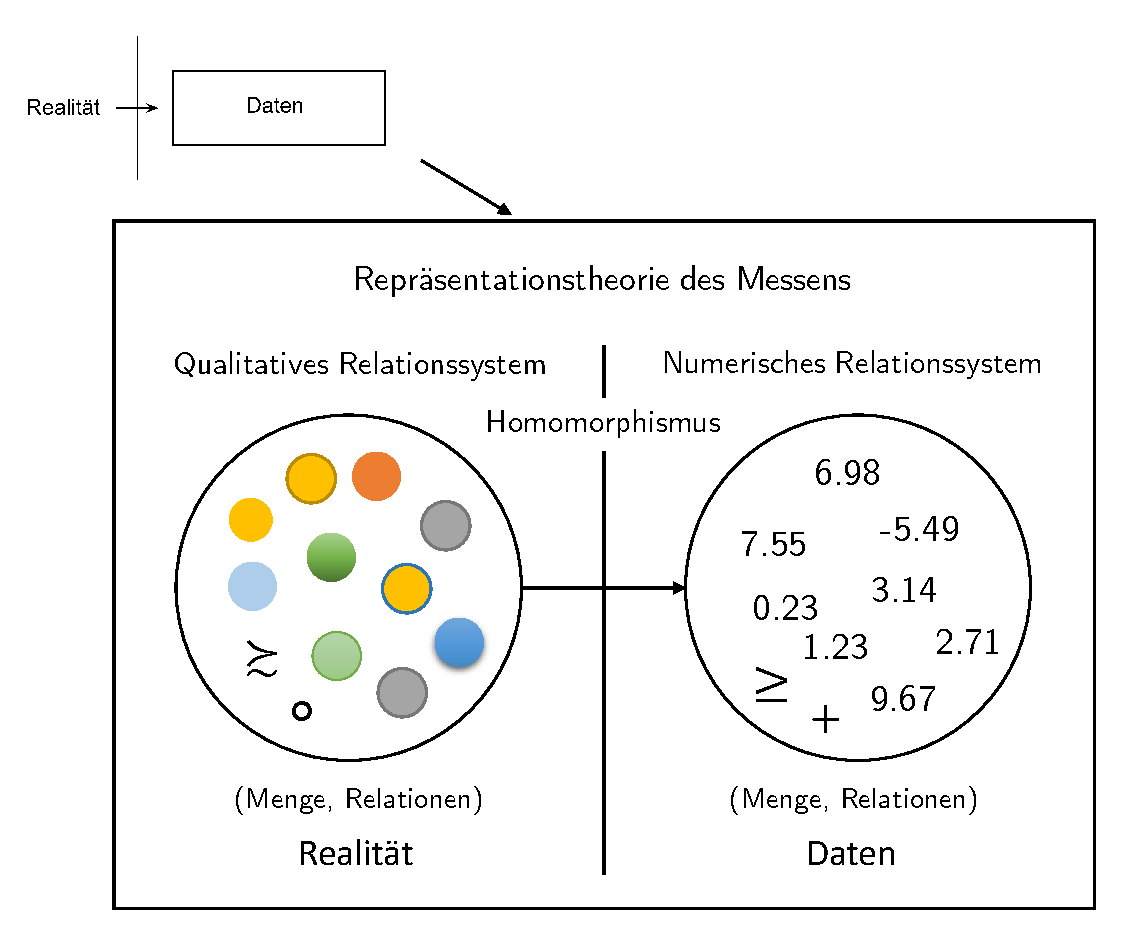
\includegraphics[width=0.8\linewidth]{5_Abbildungen/pfm_5_messtheorie} \end{center}
\end{frame}

\begin{frame}{}
\protect\hypertarget{section-2}{}
\setstretch{2.5}
\vfill
\Large

Definition

Ausgewählte Eigenschaften

Operationen

Relationssysteme

Selbstkontrollfragen \vfill
\end{frame}

\begin{frame}{}
\protect\hypertarget{section-3}{}
\setstretch{2.5}
\vfill
\Large

\textbf{Definition}

Ausgewählte Eigenschaften

Operationen

Relationssysteme

Selbstkontrollfragen \vfill
\end{frame}

\begin{frame}{Definition}
\protect\hypertarget{definition}{}
\footnotesize
\begin{definition}[Kartesische Produkte]
\justifying
$M$ und $N$ seien zwei Mengen. Dann ist das \textit{Kartesische Produkt der Mengen
$M$ und $N$} die Menge aller geordneten Tupel $(m,n)$ mit $m \in M$ und $n \in N$,
formal
\begin{equation}
M \times N := \{(m,n)|m\in M, n\in N\}
\end{equation}
Das Kartesische einer Menge $M$ mit sich selbst wird bezeichnet mit
\begin{equation}
M^2 := M \times M
\end{equation}
Seien weiterhin $M_1,...,M_n$ Mengen. Dann ist das \textit{Kartesische Produkt
der Mengen $M_1,...,M_n$} die Menge aller geordneten $n$-Tupel $(m_1,,...,m_n)$
mit $m_i \in m_i$ für $i = 1,...,n$, formal
\begin{equation}
\prod_{i=1}^n M_i := M_1 \times \cdots \times M_n := \{(m_1,...,m_n)|m_i \in M_i \mbox{ für } i = 1,...,n\}.
\end{equation}
Das $n$-fache Kartesische Produkt einer Menge $M$ mit sich selbst wird bezeichnet mit
\begin{equation}
M^n := \prod_{i=1}^n A := \{(m_1,...,m_n)|m_i \in M \mbox{ für } i = 1,...,n\}.
\end{equation}
\end{definition}
\end{frame}

\begin{frame}{Definition}
\protect\hypertarget{definition-1}{}
\footnotesize

Beispiele

\begin{enumerate}
[(1)]
\tightlist
\item
  Es sei \(M := \{1,2\}\) und \(N := \{1,2,3\}\). Dann ist \begin{align}
  \begin{split}
  M \times N
  & := \{(m,n)| m \in \{1,2\}, n \in \{1,2,3\}\}    \\
  & := \{(1,1), (1,2), (1,3), (2,1), (2,2), (2,3)\} \\
  \end{split}
  \end{align}
\item
  Es seien \(M_1 := \{a,b\}\), \(M_2 := \{c,d\}\) und
  \(M_3 := \{e,f\}\). Dann ist \begin{align}
  \begin{split}
  \prod_{i=1}^3 M_i
  & := M_1 \times M_2 \times M_3                                           \\
  & := \{(m_1,m_2,m_3)|m_1 \in M_1, m_2\in M_2, m_3 \in M_3\}              \\
  & := \{(a,c,e),(b,c,e),(a,d,e),(b,d,e),(a,c,f),(b,c,f),(a,d,f),(b,d,f)\}
  \end{split}
  \end{align}
\end{enumerate}

Bemerkungen

\begin{itemize}
\tightlist
\item
  Offenbar gilt
  \(|M_1 \times \cdots \times M_n| := \prod_{i=1}^n |M_i|\).
\item
  In der Definition von Mengen ist die Reihenfolge der Elemente
  unerheblich, bei \(n\)-Tupeln nicht.
\item
  Für Mengen gilt z.B. \(\{1,2\} = \{2,1\}\) oder \(\{a,c,e\}\) =
  \(\{c,e,a\}\).
\item
  Für geordnete Tupel gilt dagegen z.B. \((1,2)\neq (2,1)\) und
  \((a,c,e) \neq (c,e,a)\).
\end{itemize}
\end{frame}

\begin{frame}{Definition}
\protect\hypertarget{definition-2}{}
\footnotesize
\begin{definition}[$n$-stellige Relation]
\justifying
Gegeben seien $n$ Mengen $M_1,...,M_n$. Dann ist eine \textit{$n$-stellige Relation $R$ auf $M_1,...,M_n$}
definiert als eine Teilmenge des Kartesischen Produkts von $M_1,...,M_n$,
\begin{equation}
R \subseteq \prod_{i=1}^n M_i := M_1 \times \cdots \times M_n := \{(m_1,...,m_n)|m_i \in M_i, i = 1,...,n\}.
\end{equation}
\end{definition}

Bemerkungen

\begin{itemize}
\tightlist
\item
  Eine \(n\)-stellige Relation ist eine Menge von geordneten
  \(n\)-Tupeln.
\item
  Für zwei Mengen \(M_1\) und \(M_2\) ist eine \(2\)-stellige Relation
  \(R\) eine Menge von geordneten Paaren. \begin{equation}
  R = \{(m_1,m_2)|m_1 \in M_1,m_2 \in M_2\} \subset M_1 \times M_2.
  \end{equation}
\item
  Für drei Mengen \(M_1, M_2\) und \(M_3\) ist eine \(3\)-stellige
  Relation \(R\) eine Menge von geordneten Tripeln \begin{equation}
  R = \{(m_1,m_2,m_3)|m_1 \in M_1, m_2 \in M_2, m_3 \in M_3\} \subset M_1 \times M_2 \times M_3.
  \end{equation}
\item
  Die Mengen \(M_1,...,M_n\) sind nicht notwendig verschieden.
\item
  Eine zweistellige Relation auf \(M_1 \times M_2\) mit \(M_1 = M_2\),
  also \(M_1 \times M_2 = M^2\) heißt \textit{Binärrelation auf $M$}.
\item
  Wir betrachten in der Folge Binärrelationen genauer.
\end{itemize}
\end{frame}

\begin{frame}{Definition}
\protect\hypertarget{definition-3}{}
\small
\begin{definition}[Binärrelation]
\justifying
$M$ sei eine Menge. Dann heißt eine Teilmenge $R$ des Kartesischen Produkts $M \times M$
eine \textit{Binärrelation auf $M$}. Wenn für ein (geordnetes Paar) $(m,n) \in M \times M$
gilt, dass $(m \times n) \in R$ ist, so schreiben wir $m\diamond n$ und bezeichnen
die Binärrelation mit $\diamond$.
\end{definition}

Bemerkungen

\begin{itemize}
\tightlist
\item
  Es gilt \((m,n) \in R \Leftrightarrow m \diamond n\).
\item
  In seltenen Fällen schreibt man auch \(R(m,n)\) für \((m,n)\in R\).
\end{itemize}
\end{frame}

\begin{frame}{Definition}
\protect\hypertarget{definition-4}{}
\small

Beispiel (1)

\footnotesize

Es sei \(\mathbb{R}\) die Menge der reellen Zahlen. Dann ist die Menge
definiert durch \begin{equation}
R := \{(x,y)|x \ge y \mbox{ und } x,y \in \mathbb{R}\} \subset \mathbb{R}
\end{equation} eine Binärrelation auf \(\mathbb{R}\). Wir nennen diese
Relation die \(\ge\) (größer-gleich) Relation. \vfill \large \center

\begin{center}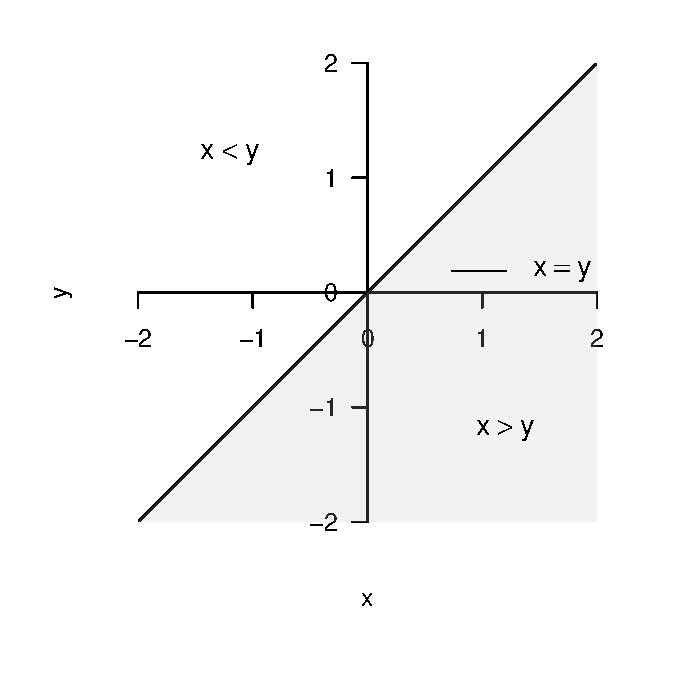
\includegraphics[width=0.5\linewidth]{5_Abbildungen/pfm_5_ge} \end{center}
\vspace{-5mm}
\center
\footnotesize

\(\{(x,y)|x \ge y \mbox{ und } x,y \in \mathbb{R}\} = - \cup\)
\textcolor{lightgray}{$\blacksquare$}
\end{frame}

\begin{frame}{Definition}
\protect\hypertarget{definition-5}{}
\small

Beispiel (2)

\footnotesize

Es sei \(M := \{a,b,c\}\) eine Menge. Dann ist \begin{equation}
M \times M = \{(a,a), (a,b), (a,c), (b,a), (b,b), (b,c), (c,a), (c,b), (c,c)\}
\end{equation} Jede Teilmenge von \(M \times M\) ist eine Relation auf
\(M\).

Zum Beispiel ist also \begin{equation}
R := \{(a,a), (b,b), (c,c)\}
\end{equation} eine Relation auf \(M\). Man schreibt hier also
\(a \diamond a\), \(b \diamond b\), \(c \diamond c\), aber auch zum
Beispiel \(a \cancel{\diamond}b\).

Eine andere Relation auf \(M\) ist \begin{equation}
R := \{(a,b), (b,c), (a,c)\}
\end{equation} Man schreibt hier entsprechend \(a \diamond b\),
\(b \diamond c\), \(a \diamond c\), aber zum Beispiel auch
\(a \cancel{\diamond}a\).
\end{frame}

\begin{frame}{}
\protect\hypertarget{section-4}{}
\setstretch{2.5}
\vfill
\Large

Definition

\textbf{Ausgewählte Eigenschaften}

Operationen

Relationssysteme

Selbstkontrollfragen \vfill
\end{frame}

\begin{frame}{Ausgewählte Eigenschaften}
\protect\hypertarget{ausgewuxe4hlte-eigenschaften}{}
\small
\begin{definition}[Reflexivität]
\justifying
Eine Binärrelation $R$ auf eine Menge $M$ heißt \textit{reflexiv}, wenn für
jedes $m \in M$ gilt, dass $(m,m)\in R$ ist, wenn also $m \diamond m$ gilt.
\end{definition}

\footnotesize

Bemerkungen und Beispiele

\begin{itemize}
\tightlist
\item
  Die \(\ge\) Relation auf \(\mathbb{R}\) is reflexiv, weil für alle
  \(x \in \mathbb{R}\) gilt, dass \(x \ge x\).
\item
  Für \(M := \{a,b\}\) ist \begin{equation}
  R := \{(a,a), (a,b), (b,a), (b,b)\}
  \end{equation} eine reflexive Relation auf \(M\), weil für \(a \in M\)
  und \(b \in M\) gilt, dass \((a,a)\) und \((b,b)\) in \(R\) sind.
\item
  Für \(M := \{a,b\}\) ist \begin{equation}
  R := \{(a,a), (a,b), (b,a)\}
  \end{equation} keine reflexive Relation auf \(M\), weil
  \((b,b)\notin R\).
\end{itemize}
\end{frame}

\begin{frame}{Ausgewählte Eigenschaften}
\protect\hypertarget{ausgewuxe4hlte-eigenschaften-1}{}
\footnotesize
\begin{definition}[Irreflexivität]
\justifying
Eine Binärrelation $R$ auf eine Menge $M$ heißt \textit{reflexiv}, wenn für
jedes $m \in M$ gilt, dass $(m,m)\notin R$ ist, wenn also $m \cancel{\diamond} m$ gilt.
\end{definition}

Bemerkungen und Beispiele

\begin{itemize}
\tightlist
\item
  Die \(>\) Relation auf \(\mathbb{R}\) is irreflexiv, denn für kein
  \(x \in \mathbb{R}\) gilt, dass \(x > x\).
\item
  Für \(M := \{a,b\}\) ist \begin{equation}
  R := \{(a,b), (b,a)\}
  \end{equation} eine irreflexive Relation auf \(M\), weil für
  \(a \in M\) und \(b \in M\) gilt, dass \((a,a)\notin R\) und
  \((b,b)\notin R\) sind.
\item
  Irreflexiv und nicht reflexiv sind nicht identisch: eine Relation ist
  schon dann nicht reflexiv, wenn es nur ein \(m \in M\) mit
  \((m,m)\notin R\) gibt, allerdings ist sie nur dann irreflexiv, wenn
  dies tatsächlich für alle \(m \in M\) gilt.
\item
  Sei zum Beispiel \(M := \mathbb{R}^2\) und \begin{equation}
  R := \{(x,y)|y = x^2\}
  \end{equation} Dann gilt \((1,1) \in R\), weil \(1 = 1^2\), aber
  \((2,2) \notin R\), weil \(2 \neq 2^2\). Also ist \(R\) auf
  \(\mathbb{R}^2\) weder reflexiv noch irreflexiv.
\end{itemize}
\end{frame}

\begin{frame}{Ausgewählte Eigenschaften}
\protect\hypertarget{ausgewuxe4hlte-eigenschaften-2}{}
\small
\begin{definition}[Symmetrie]
\justifying
Eine Binärrelation $R$ auf einer Menge $M$ heißt \textit{symmetrisch}, wenn für alle
$(m,n)\in R$ folgt, dass auch $(n,m)\in R$ ist, wenn also aus $m \diamond n$ folgt,
dass $n \diamond n$ gilt.
\end{definition}

\footnotesize

Bemerkungen und Beispiele

\begin{itemize}
\tightlist
\item
  Die \(\ge\) Relation auf \(\mathbb{R}\) ist nicht symmetrisch, weil
  aus \(x \ge y\) nicht notwendigerweise folgt, dass \(y \ge x\): es
  kann ja auch \(x>y\) gelten, dann gilt \(y \ge x\) aber nicht.
\item
  Für \(M := \{a,b\}\) ist \begin{equation}
  R := \{(a,b), (b,a)\}
  \end{equation} eine symmetrische Relation auf \(M\), weil
  \begin{align}
  \begin{split}
  (a,b) \in R & \Rightarrow (b,a) \in R \\
  (b,a) \in R & \Rightarrow (a,b) \in R \\
  \end{split}
  \end{align}
\item
  Für \(M := \{a,b\}\) ist \begin{equation}
  R := \{(a,a), (a,b), (b,b)\}
  \end{equation} keine symmetrische Relation auf \(M\), weil
  \((a,b) \in R\), aber \((b,a) \notin R\).
\end{itemize}
\end{frame}

\begin{frame}{Ausgewählte Eigenschaften}
\protect\hypertarget{ausgewuxe4hlte-eigenschaften-3}{}
\small
\begin{definition}[Transitivität]
\justifying
Eine Binärrelation $R$ auf einer Menge $M$ heißt \textit{transitiv}, wenn für alle
$m,n\in R$ gilt, dass aus $(m,n)\in R$ und $(n,p)\in R$ folgt, dass $(m,p) \in R$ ist,
wenn also aus $m \diamond n$ und $n \diamond p$ folgt, dass $m \diamond p$ gilt.
\end{definition}

\footnotesize

Beispiele

\begin{itemize}
\tightlist
\item
  Die \(\ge\) Relation auf \(\mathbb{R}\) ist transitiv, denn aus
  \(x \ge y\) und \(y \ge z\) folgt, dass \(x \ge z\).
\item
  Auf \(M := \{a,b,c\}\) ist \begin{equation}
  R := \{(a,b), (b,c), (a,c)\}
  \end{equation} eine transitive Relation, weil neben \((a,b) \in R\)
  und \((b,c) \in R\) auch \((a,c) \in R\) gilt.
\item
  Für \(M := \{a,b,c\}\) ist \begin{equation}
  R := \{(a,b), (b,c), (a,c)\}
  \end{equation} keine transitive Relation auf \(M\), weil trotz
  \((a,b) \in R\) und \((b,c) \in R\) nicht \((a,c) \in R\) gilt.
\end{itemize}
\end{frame}

\begin{frame}{Ausgewählte Eigenschaften}
\protect\hypertarget{ausgewuxe4hlte-eigenschaften-4}{}
\small
\begin{definition}[Negative Transitivität]
\justifying
Eine Binärrelation $R$ auf einer Menge $M$ heißt \textit{negativ transitiv}, wenn für alle
$m,n\in R$ gilt, dass aus $(m,n)\notin R$ und $(n,p)\notin R$ folgt, dass $(m,p) \notin R$ ist,
wenn also aus $m \cancel{\diamond} n$ und $n \cancel{\diamond} p$ folgt, dass $m \cancel{\diamond} p$ gilt.
\end{definition}

\footnotesize

Beispiele

\begin{itemize}
\tightlist
\item
  Die \(>\) Relation auf \(\mathbb{R}\) ist negativ transitiv, denn aus
  \(x \cancel{>} y\) (also \(x \le y\)) und \(y \cancel{>} z\) (also
  \(y \le z\)), folgt \(x \le z\), also \(x \cancel{>} z\).
\item
  Auf \(M := \{a,b,c\}\) ist \begin{equation}
  R := \{(a,b), (b,c), (a,c)\}
  \end{equation} negativ transitiv, denn hier folgt zum Beispiel aus
  \((c,b) \notin R\) und \((b,a) \notin R\), dass \((c,a) \notin R\).
  Zum vollständigem Nachweis der negativen Transitität müsste dies für
  alle möglichen relevanten Paare nachgewiesen werden.
\item
  Dagegen ist auf \(M := \{a,b,c\}\)\\
  \begin{equation}
  R := \{(a,b), (b,c), (c,a)\}
  \end{equation} nicht negativ transitiv, denn trotz \((b,a) \notin R\)
  und \((a,c) \notin R\) gilt hier \((b,c) \in R\).
\end{itemize}
\end{frame}

\begin{frame}{}
\protect\hypertarget{section-5}{}
\setstretch{2.5}
\vfill
\Large

Definition

Ausgewählte Eigenschaften

\textbf{Operationen}

Relationssysteme

Selbstkontrollfragen \vfill
\end{frame}

\begin{frame}{Operationen}
\protect\hypertarget{operationen}{}
\small
\begin{definition}[Relationsdefinition von Funktionen]
\justifying
$D$ und $Z$ seien Mengen. Eine Binärrelation $f$ auf $D \times Z$ heißt \textit{Funktion
(oder Abbildung) von $D$ nach $Z$}, wenn $f$ folgende Eigenschaften hat:
\begin{enumerate}
\item[(1)] Für alle $x \in D$ gibt es ein $y \in Z$, so dass $(x,y) \in f$.
\item[(2)] Wenn $(x,y)\in f$ und $(x,y') \in f$ sind, so folgt $y = y'$.
\end{enumerate}
\end{definition}
\footnotesize

Bemerkungen

\begin{itemize}
\tightlist
\item
  \justifying Eine Funktion wird hier betrachtet als eine Menge von
  geordneten Paaren \begin{equation}
  f := \{(x,y)|x\in D, y\in Z\} \subseteq D \times Z
  \end{equation}
\item
  Eigenschaft (1) besagt, dass eine Funktion jedem Element in \(D\)
  mindestens ein Element in \(Z\) zuordnet.
\item
  Eigenschaft (2) besagt, dass eine Funktion jedem Element in \(D\)
  höchstens ein Element in \(Z\) zuordnet.
\item
  Zusammen besagen (1) und (2) also, dass eine Funktion jedem
  \(x \in D\) genau ein \(y \in Z\) zuordnet.
\item
  Unsere Notation von Funktionen bleibt von der Relationsdefinition von
  Funktionen unberührt, wir schreiben weiterhin \(f : D \to Z\) dafür,
  dass \(f\) eine Funktion (Abbildung) von \(D\) nach \(Z\) ist und
  bezeichnen das zu \(x \in D\) eindeutig bestimmte \(y \in Z\) als
  \(f(x):=y\).
\item
  Die Relationsdefinition von Funktionen definiert Funktionen als
  Mengen, vermeidet den undefinierten Begriff der ``Vorschrift'' und
  gibt der Mathematik somit eine rein mengentheoretische Grundlage.
\end{itemize}
\end{frame}

\begin{frame}{Operationen}
\protect\hypertarget{operationen-1}{}
\small
\begin{definition}[Operation]
$M$ sei eine Menge. Eine \textit{Operation (oder Verknüpfung)} $\circ$ auf $M$ ist eine
Funktion der Form
\begin{equation}
\circ : N \subseteq M \times M \to M, (m,n) \mapsto \circ((m,n))).
\end{equation}
\end{definition}
\footnotesize

Bemerkungen

\begin{itemize}
\tightlist
\item
  Die Einschränkung von \(M \times M\) auf \(N \subseteq M \times M\)
  dient dem Realitätsanspruch extensiver Strukturen.
\item
  Siehe dazu auch Krantz and Suppes (1971), S. 81-82.
\item
  Im numerischen Kontext ist meist \(N = M \times M\).
\end{itemize}
\end{frame}

\begin{frame}{Operationen}
\protect\hypertarget{operationen-2}{}
\small

Beispiele

\footnotesize

\(\bullet\) Eine vertraute Operation ist die Addition natürlicher Zahlen
\begin{equation}
+ : \mathbb{N} \times \mathbb{N} \to \mathbb{N}, (m,n) \mapsto +((m,n)) := m + n.
\end{equation} \(\bullet\) Eine andere vertraute Operation ist die
Multiplikation ganzer Zahlen, \begin{equation}
\cdot : \mathbb{Z} \times \mathbb{Z} \to \mathbb{Z}, (m,n) \mapsto \cdot((m,n)) := mn.
\end{equation} \(\bullet\) Für eine Menge \(N\) und die Menge
\begin{equation}
M := \{f : N \to N| f \mbox{ ist eine Funktion}\}
\end{equation} \(\,\,\,\) ist die Verknüpfung von Funktionen eine
Operation auf \(M\), \begin{equation}
\circ : M \times M \to M, (f,g) \mapsto \circ((f,g)) := f \circ g \mbox{ mit } (f \circ g)(m) := f(g(m)) \mbox{ für alle } m \in M.
\end{equation} \(\bullet\) Eine Operation ist eine 3-stellige Relation
\(R\) auf einer Menge \(M\) der Form \begin{equation}
R = \{(m,n, m\circ n)|m,n,m\circ n \in M\} \subseteq M \times M \times M
\end{equation} \(\,\,\,\) Allerdings ist nicht jede 3-stellige Relation
\(R\) auf einer Menge \(M\) eine Operation
\end{frame}

\begin{frame}{Operationen}
\protect\hypertarget{operationen-3}{}
\small

Beispiele (fortgeführt)

\footnotesize

\(\bullet\) Sei zum Beispiel \(M := \{1,2,3\}\). Dann entspricht die
Operation \begin{equation}
\circ : M \times M \to M,
(m,n) \mapsto \circ((m,n)) :=
\begin{cases}
1 & \mbox{ wenn } a + b \mbox{ gerade ist} \\
2 & \mbox{ wenn } a + b \mbox{ ungerade ist} \\
\end{cases}.
\end{equation} \(\,\,\,\) der 3-stelligen Relation \begin{equation}
R = \{(1,1,1), (1,2,2), (1,3,1), (2,1,2), (2,2,1), (2,3,2), (3,1,1), (3,2,2), (3,3,1)\}
\end{equation} \(\bullet\) Sei zum Beispiel wiederum \(M := \{1,2,3\}\)
und die 3-stellige Relation \(R\) definiert als \begin{equation}
R := \{(1,1,1), (1,2,2), (1,3,1), (2,1,2), (2,2,1), (2,3,2), (3,1,1), (3,2,2), (1,3,2)\}.
\end{equation} \(\,\,\,\) Dann gilt sowohl \((1,3,1) \in R\) und
\((1,3,2) \in R\), also in Operationschreibweise \begin{equation}
(1,3) \mapsto \circ((1,3)) := 1 \mbox{ und } (1,3) \mapsto \circ((1,3)) := 2.
\end{equation} \(\,\,\,\) Dann ist \(\circ\) aber keine Funktion, weil
eine Funktion jedem Element der Definitionsmenge nur höchstens ein
Element

\(\,\,\,\) der Zielmenge zuordnet und nicht zwei.
\end{frame}

\begin{frame}{}
\protect\hypertarget{section-6}{}
\setstretch{2.5}
\vfill
\Large

Definition

Ausgewählte Eigenschaften

Operationen

\textbf{Relationssysteme}

Selbstkontrollfragen \vfill
\end{frame}

\begin{frame}{Relationssysteme}
\protect\hypertarget{relationssysteme}{}
\small
\begin{definition}[Relationssystem]
\justifying
$M$ sei eine Menge, $R_1,...,R_p$ seien Relationen auf $M$ und $\circ_1,...,\circ_q$
seien Operationen auf $M$. Dann wird das $(1 + p + q)$-Tupel
\begin{equation}
\mathcal{M} := (M,R_1,...,R_p, \circ_1,...,\circ_q)
\end{equation}
ein \textit{Relationssystem} genannt. Für $M := \mathbb{R}$ heißt ein Relationssystem
ein \textit{numerisches Relationssystem}. Der \textit{Typ eines Relationssystems}
ist eine (endliche) Folge $(r_1,...,r_p,q)$ der Länge $p+1$, für die gilt, dass für alle
$i = 1,...,p$ $r_i$ gleich $\rho$ ist, wenn $R_i$ eine $\rho$-stellige Relation ist.
\end{definition}
\footnotesize

Bemerkungen

\begin{itemize}
\tightlist
\item
  Da \(\circ_1,...,\circ_q\) Binärrelationen sind, könne man auch
  \(\mathcal{M} := (M,R_1,...,R_{p+q})\) schreiben.
\item
  Der Relationstyp \((2,3,2)\) eines Relationssystems \(\mathcal{M}\)
  besagt, dass auf der Menge \(M\) eine 2-stellige und eine 3-stellige
  Relation, sowie zwei Operationen definiert sind.
\end{itemize}
\end{frame}

\begin{frame}{Relationssystem}
\protect\hypertarget{relationssystem}{}
\vspace{2mm}
\setstretch{1.2}
\small

Beispiele für (qualitative) Relationssysteme \footnotesize

\begin{enumerate}
[(1)]
\item
  \(M\) sei eine Menge von Objekten und es sei \begin{equation}
  R := \{(m,n)| m \mbox{ ist wärmer als } n\} \subseteq  M\times M.
  \end{equation} Dann ist \(\mathcal{M} := (M,R)\) ein Relationssystem
  vom Typ \((2,0)\).
\item
  \(M\) sei eine Menge von Entscheidungsoptionen und es sei
  \begin{equation}
  R := \{(m,n)| m \mbox{ wird präferiert über } n\} \subseteq  M\times M
  \end{equation} Dann ist \(\mathcal{M} := (M,R)\) ein Relationssystem
  vom Typ \((2,0)\).
\item
  \(M\) sei eine Menge von Objekten und es sei \begin{equation}
  R := \{(m,n)| m \mbox{ ist schwerer als } n\} \subseteq  M\times M
  \end{equation} und \begin{equation}
  \circ : M \times M \to M, (m,m) \mapsto \circ((m,n)) := \mbox{Die physische Kombination von } m \mbox{ und } n.
  \end{equation} Dann ist \(\mathcal{M} := (M,R,\circ)\) ein
  Relationssystem vom Typ \((2,1)\).
\end{enumerate}

\small

Beispiele für numerische Relationssysteme \footnotesize

\begin{enumerate}
[(1)]
\tightlist
\item
  \(\mathcal{N} := (\mathbb{R},>)\) ist ein numerisches Relationsystem
  vom Typ (2,0).
\item
  \(\mathcal{N} := (\mathbb{R},>,\ge)\) ist ein numerisches
  Relationsystem vom Typ (2,2,0).
\item
  \(\mathcal{N} := (\mathbb{R},>,\ge, +)\) ist ein numerisches
  Relationsystem vom Typ (2,2,1).
\item
  \(\mathcal{N} := (\mathbb{R},>,\ge, +, \cdot)\) ist ein numerisches
  Relationsystem vom Typ (2,2,2).
\end{enumerate}
\end{frame}

\begin{frame}{}
\protect\hypertarget{section-7}{}
\setstretch{2.5}
\vfill
\Large

Definition

Ausgewählte Eigenschaften

Operationen

Relationssysteme

\textbf{Selbstkontrollfragen} \vfill
\end{frame}

\begin{frame}{Selbstkontrollfragen}
\protect\hypertarget{selbstkontrollfragen}{}
\setstretch{2}

\footnotesize

\begin{enumerate}
\tightlist
\item
  Definieren Sie das Kartesische Produkt zweier Mengen.
\item
  Definieren Sie das Kartesische Produkt dreier Mengen.
\item
  Definieren Sie den Begriff der Binärrelation.
\item
  Definieren Sie den Begriff einer dreistelligen Relation.
\item
  Erläutern Sie die \(\ge\) Relation.
\item
  Definieren Sie den Begriff der reflexiven Binrärelation.
\item
  Definieren Sie den Begriff der irreflexiven Binrärelation.
\item
  Was ist der Unterschied zwischen einer nicht reflexiven und einer
  irreflexiven Relation?
\item
  Definieren Sie den Begriff einer symmetrischen Binärrelation.
\item
  Definieren Sie den Begriff einer transitiven Binärrelation.
\item
  Definieren Sie den Begriff einer negativ-transitiven Binärrelation.
\item
  Geben Sie die Relationsdefinition einer Funktion wieder.
\item
  Definieren Sie den Begriff der Operation.
\item
  Definieren Sie den Begriff des Relationssystems.
\item
  Geben Sie ein Beispiel für ein qualitatives Relationssytem.
\item
  Geben Sie ein Beispiel für ein numerisches Relationssystem.
\end{enumerate}
\end{frame}

\begin{frame}{Referenzen}
\protect\hypertarget{referenzen}{}
\footnotesize

\hypertarget{refs}{}
\begin{CSLReferences}{1}{0}
\leavevmode\vadjust pre{\hypertarget{ref-krantz_1971}{}}%
Krantz, David H., and Patrick Suppes, eds. 1971. \emph{Foundations of
Measurement}. {New York}: {Academic Press}.

\end{CSLReferences}
\end{frame}

\end{document}
